% id: 0174
% book: 쎈 중3-2 수학 · 02 삼각비의 활용
% section: 유형 01 직각삼각형의 변의 길이
% figure: tikz:fig-0174
% answer: (1) $4.32$ (2) $5.76$
% answer_source: 답지
% variant_level: 0 (원본 전사)
% 이 파일은 build.mjs 가 items.json 에서 만든다. 고칠 때는 items.json 을 고친다.
\smash{\raisebox{1.5mm}{\dmkichul{쎈 중3-2 수학 0174번 · 36쪽 · 서술형}}}
\noindent\begin{minipage}[t]{0.58\linewidth}\vspace{0pt}\raggedright 오른쪽 그림과 같이 $\seg{AB}=8$, $\angle\pt{B}=33^\circ$, $\angle\pt{C}=49^\circ$인 $\triangle\pt{ABC}$에서 $\seg{AH}\perp\seg{BC}$일 때, 다음 선분의 길이를 구하시오. \cond{$\sin 33^\circ=0.54$, $\sin 49^\circ=0.75$로 계산한다.}\end{minipage}\hfill\begin{minipage}[t]{0.4\linewidth}\vspace{0pt}\centering \resizebox{\ifdim\width>\linewidth\linewidth\else\width\fi}{!}{% 0174(본책 36쪽) — △ABC(AB=8, ∠B=33°, ∠C=49°), AH⊥BC. 스캔 삽화를 TikZ 로 다시 그림. 답(AH·AC)은 적지 않는다.
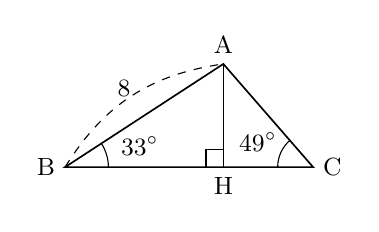
\begin{tikzpicture}[line width=0.6pt]
  \coordinate (B) at (0,0); \coordinate (A) at (2.01,1.31); \coordinate (H) at (2.01,0); \coordinate (C) at (3.15,0);
  \draw (A) -- (B) -- (C) -- cycle;
  \draw (A) -- (H);
  \draw[line width=0.4pt] (1.79,0) -- (1.79,0.22) -- (2.01,0.22);
  \draw[line width=0.4pt] (0.55,0) arc[start angle=0, end angle=33, radius=0.55];
  \node[font=\small] at (0.95,0.27) {$33^\circ$};
  \draw[line width=0.4pt] (2.7,0) arc[start angle=180, end angle=131, radius=0.45];
  \node[font=\small] at (2.45,0.32) {$49^\circ$};
  \draw[dashed, line width=0.4pt] (B) to[bend left=25] (A);
  \node[font=\small] at (0.75,1.0) {$8$};
  \node[font=\small, above] at (A) {A};
  \node[font=\small, left] at (B) {B};
  \node[font=\small, right] at (C) {C};
  \node[font=\small, below] at (H) {H};
\end{tikzpicture}
}\end{minipage}\par
\dmsubprob{1} $\seg{AH}$
\dmsubprob{2} $\seg{AC}$
